\begin{figure}[t!]
\vspace*{-2\baselineskip}
\centering
\begin{subfigure}[t]{0.45\textwidth}
\centering
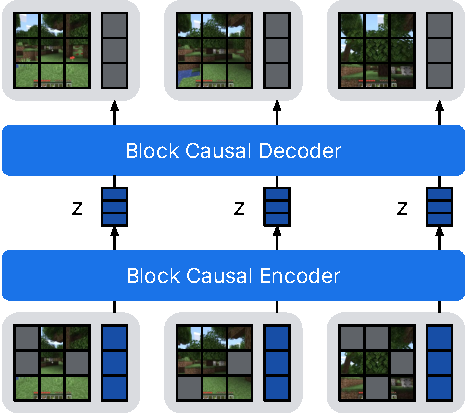
\includegraphics[height=2.4in]{figures/method/tok}
\caption{Causal Tokenizer}
\end{subfigure}%
\hfill%
\begin{subfigure}[t]{0.45\textwidth}
\centering
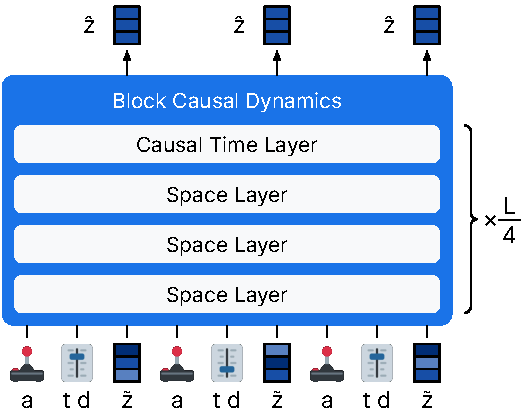
\includegraphics[height=2.5in]{figures/method/dyn}
\caption{Interactive Dynamics}
\end{subfigure}
\caption{World model design.
\method consists of a causal tokenizer and an interactive dynamics model, which both use the same block-causal transformer architecture.
The tokenizer encodes partially masked image patches and latent tokens, squeezes the latents through a low-dimensional projection with tanh activation, and decodes the patches.
It uses causal attention to achieve temporal compression while allowing frames to be decoded one by one.
The dynamics model operates on the interleaved sequence of actions, shortcut noise levels and step sizes, and tokenizer representations.
It denoises representations via a shortcut forcing objective.
After pretraining, the world model is finetuned into an agent by inserting task tokens into the dynamics transformer and predicting actions, rewards, and values from them.
}
\label{fig:model}
\end{figure}